A system is judged by the quality of the services it offers and its ability to function reliably. Even though the reliability of operating systems has been studied for several decades, it remains a major concern today. The characteristics of the operating systems which make them unstable are size and complexity. 
\\[3mm]
Coverity's analysis of the Linux kernel code found 1000 bugs in the source code of version 2.4.1 of the Linux kernel, and 950 bugs still in 2.6.9. This study also shows that 53\% of the bugs are present in the device driver portion of the kernel~\cite{coveritykernel}. 
\\[3mm]
In order to protect against bugs, operating systems provide protection mechanisms. These protection mechanisms protect resources such as memory and CPU.
Memory protection is the protection mechanism provided in a Linux kernel. Memory protection is a way to control memory access rights. It prevents a user process from accessing memory that has not been allocated to it. It prevents a bug within a user process from affecting other processes, or the operating system~\cite{denning1970virtual, Galvin}. However, kernel modules do not have the same level of protection the user level applications have. In the Linux kernel, any portion of the kernel can access, and potentially, overwrite kernel data structures used by unrelated components. Such non-existent isolation between kernel components can cause a bug in a device driver to corrupt the memory of other kernel components, which in turn may lead to a system crash. Thus, an underlying cause of unreliability in operating systems is the lack of isolation between device drivers and a Linux kernel.

\section {Problem Statement}
\label{sec:problem}
In the past, virtualization based solutions, which were intended to increase the reliability of a system, were proposed by LeVasseur et. al.~\cite{LeVasseur04UnmodifiedDriverReuse} and Fraser et. al.~\cite{Fraser04safehardware}. Frazer et. al. proposed the Xen isolated driver domain. In a virtualized environment, virtual machines are unaware of and isolated from the other virtual machines. Malfunctioning of one virtual machine cannot spread to the others. Hence, use of virtual machines provide extremely good fault isolation. 
\\[3mm]
In a virtualized environment, all virtual machines run as separate guest domains in different address spaces. The virtualization based solutions mentioned above exploit the memory protection between these guest domains. They improve the reliability of the system by executing device drivers and the kernel in separate virtual machines. Xen hypervisor provides a platform to the isolate device driver from the monolithic kernel called the isolated driver domain based on a split device driver model~\cite{driverdomain}.
\\[3mm]
The Xen virtual machine monitor (VMM) does not include device drivers for all the devices, adding support for all the devices would be a duplication of effort. Instead, Xen delegates hardware support to guests. The guest typically runs in a privileged domain, although it is possible to delegate hardware to guests in other domains. The model in which hardware support is delegated to a guest is called a split device driver model~\cite{Chisnall:2007:DGX:1407351}. Xen uses the same split device driver model in the isolated driver domain as shown in the figure~\ref{fig:xen-split}.
\begin{figure}[!ht]
\centering
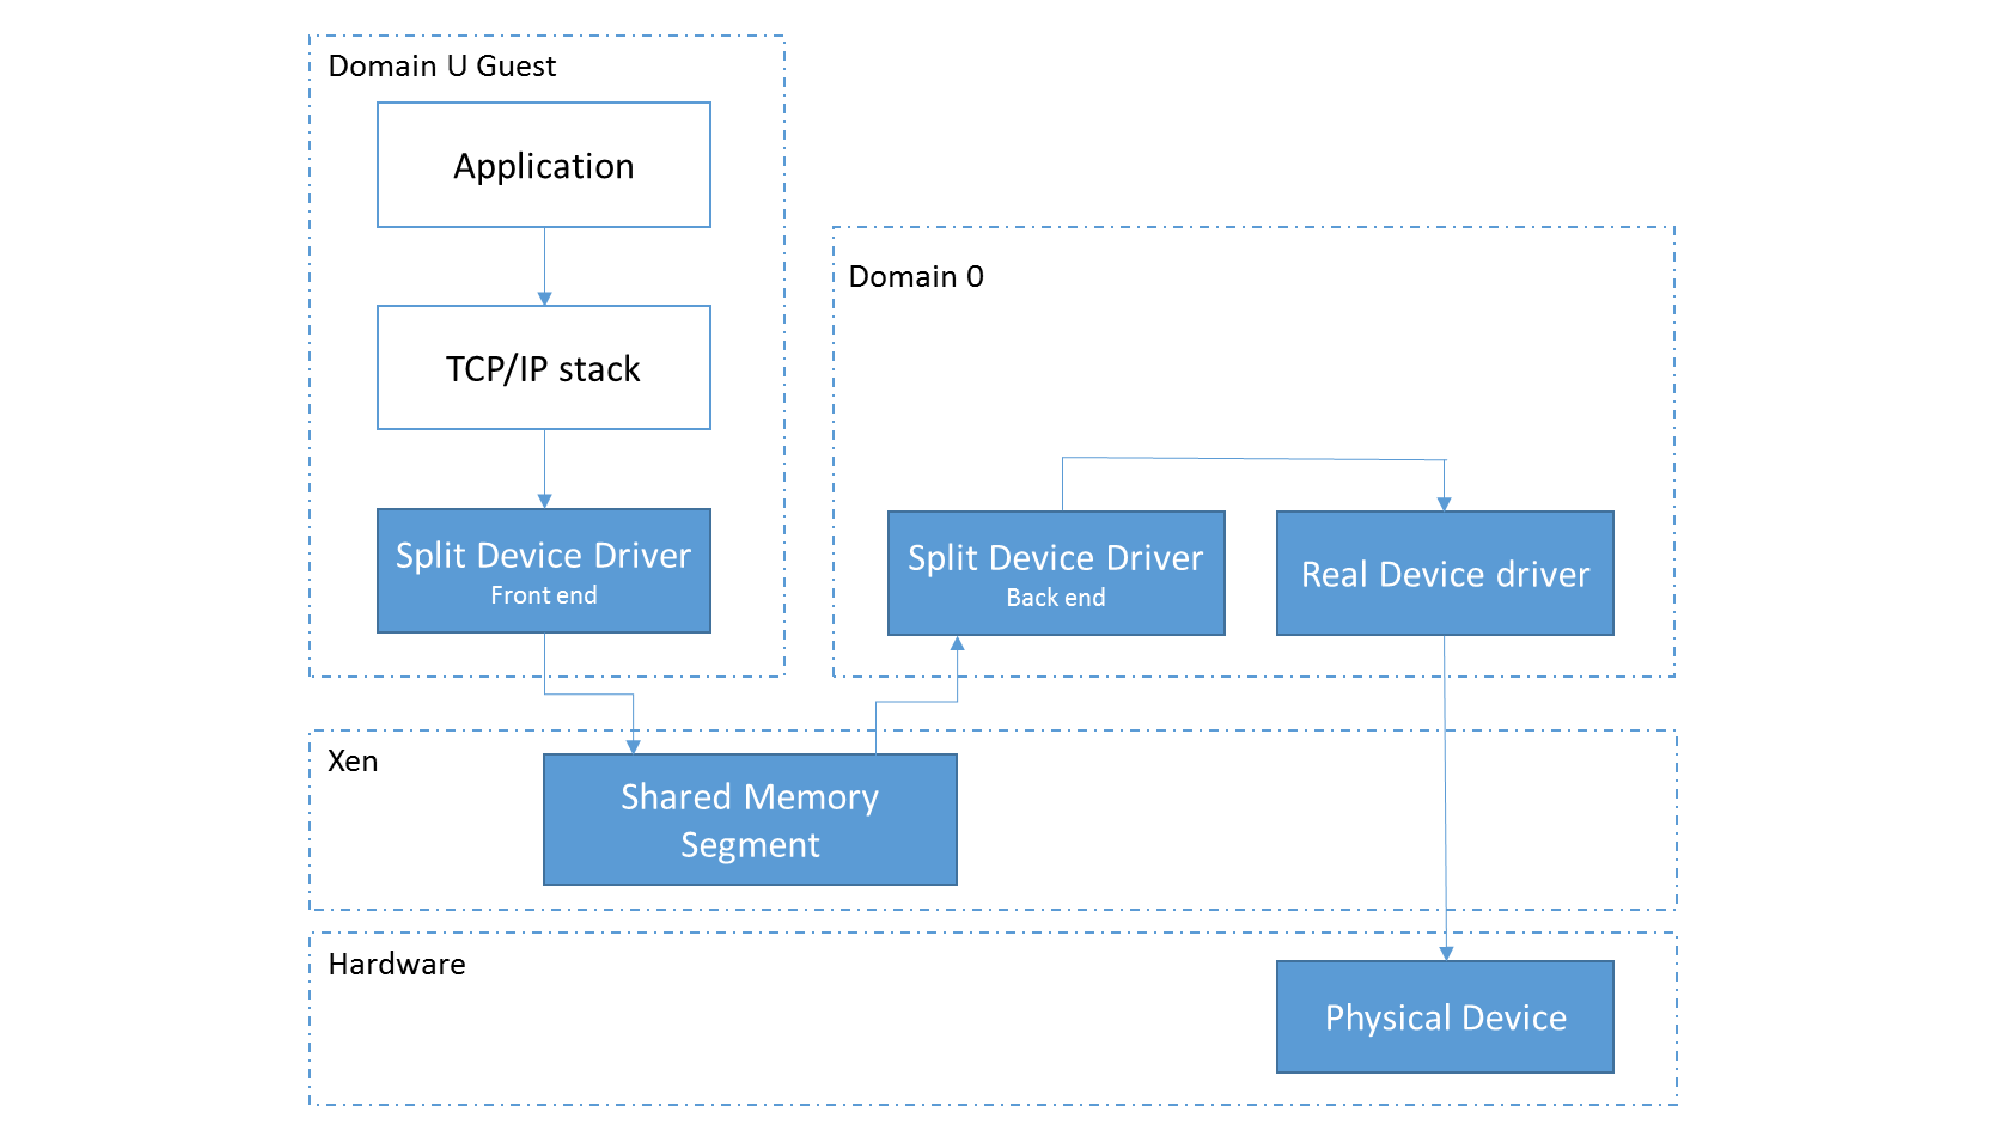
\includegraphics[scale=.50]{xen-split-tcp.pdf}
\caption{Split device driver model}
\label{fig:xen-split}
\end{figure}
Xen has a frontend driver in the guest domain and a backend driver in the driver domain. The frontend and the backend driver transfer data between domains over a channel that is provided by the Xen VMM. Within the driver domain, the backend driver is used to de-multiplex incoming data to the device and to multiplex outgoing data between the device and the guest domain~\cite{driverdomain}.
\\[3mm]
The Xen's isolated driver domain follows the split device driver architecture of Xen VMM. In the isolated driver domain, user applications and a kernel are executed in a guest domain, and a device driver is executed in a driver domain. As a result, a device driver is isolated from the Linux kernel, making it impossible for the device driver to corrupt kernel data structures in the virtual machine running user applications. 
\\[3mm]
Despite the advances in virtualization technology, the overhead of communication between guest domain and driver domain significantly affects the performance of applications~\cite{barham2003xen, Sugerman:2001:VID:647055.715774, Menon:2006:ONV:1267359.1267361}. The Xen's isolated driver domain follows an interrupt based approach in the communication channel~\cite{barham2003xen}. In this communication model, frontend and backend notifiy each other of the receipt of a service request and corresponding responses by sending an interrupt. The Xen hypervisor needs to schedule the other domain to deliver the interrupt, which might need a context switch~\cite{barham2003xen}. The context switch can cause an unavoidable system overhead~\cite{Li:2007:QCC:1281700.1281702, Mogul:1991:ECS:106973.106982}. The interrupt based notification system might cause an overhead in the communication channel of the isolated driver domain. 

\section {Proposed Solution}

In this thesis, we propose and evaluate an optimization for improving the performance of the communication between guest domain and driver domain. We propose a solution in which a thread in the backend driver spins for the service requests, and the frontend driver spins for the availability of the corresponding responses. Multiprocessors have better concurrency than single core processors. On multi core processors, spinlocks have better performance than uniprocessor system. On the other hand, a context switch takes a significant amount of time, so it is more efficient for each process to simply spin while waiting for a resource in a multiprocessor environment. Since our solution follows a spinlock based approach, it performs better than the approach used in the original implementation.
\\[3mm]
The source code for isolated driver domain is not available in the open source Xen hypervisor code. As explained in the Section~\ref{sec:problem}, isolated driver domain uses Xen's split device driver approach~\cite{Fraser04safehardware}. In this thesis, we re-implement the Xen's isolated driver domain, we refer to our implementation as Isolated Device Driver (IDDR). Our solution to improve the performance of the Xen isolated driver domain is implemented over the IDDR base code.
\\[3mm]
The performance of the system is evaluated for block devices such as ramdisk device, loop device, and SATA disk. The block device is formatted with a file system and the IDDR system is evaluated by measuring the performance of the system with fileIO/SysBench benchmark. The integrity of the system is checked by executing dd read/write, with and without read ahead, file system tests on the variety of block devices. The evaluation of our solution shows that the performance of the system can be improved by avoiding the context switches in the communication channel. 
\pagebreak
\section{Core Contributions}
The core contributions of this project are listed below: 
\begin{enumerate}
\item Re-implementation of the Xen's isolated driver domain - Isolated Device Driver (IDDR).
\item Improvement in the performance of the IDDR by implementing the thread based communication channel instead of the interrupt based communication channel. 
\item Our performance comparison of the thread based IDDR and interrupt based IDDR.
\end{enumerate}
\section {Organization}
This section gives the organization and roadmap of the thesis.
\begin{enumerate}
\item Chapter 2 gives the background on Processes, Threads, Memory Protection, Virtualization, Hypervisor and Inter-domain Communication.
\item Chapter 3 gives the introduction to design of the system to isolate device driver. 
\item Chapter 4 discusses the detailed design and implementation to isolate the device driver. 
\item Chapter 5 evaluates the performance of the Independent device driver with different designs.
\item Chapter 6 reviews the related work in the area of kernel fault tolerance.
\item Chapter 7 concludes the report and lists the topics where this work can be extended.
\end{enumerate}
\pagebreak
\ifbool{toShowBibliography}{\bibliography{references}}{}